\listoffigures
\newpage

\begin{center}
    \subsection{Telas do Gerente}
    \begin{figure}[!htp]
        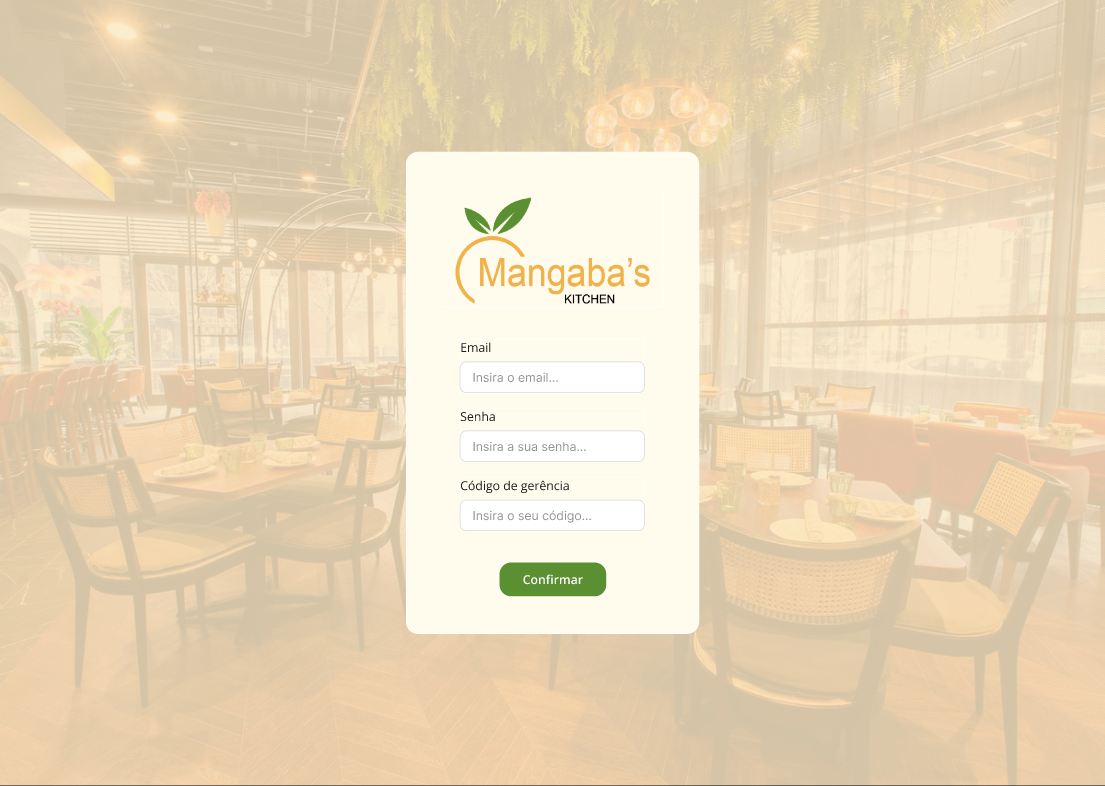
\includegraphics[width=1\textwidth]{imagens-template/Layout_Gerente_2638.png} 
        \caption{Tela de login do gerente.}
    \end{figure}
    \newpage
    \begin{figure}[!htp]
        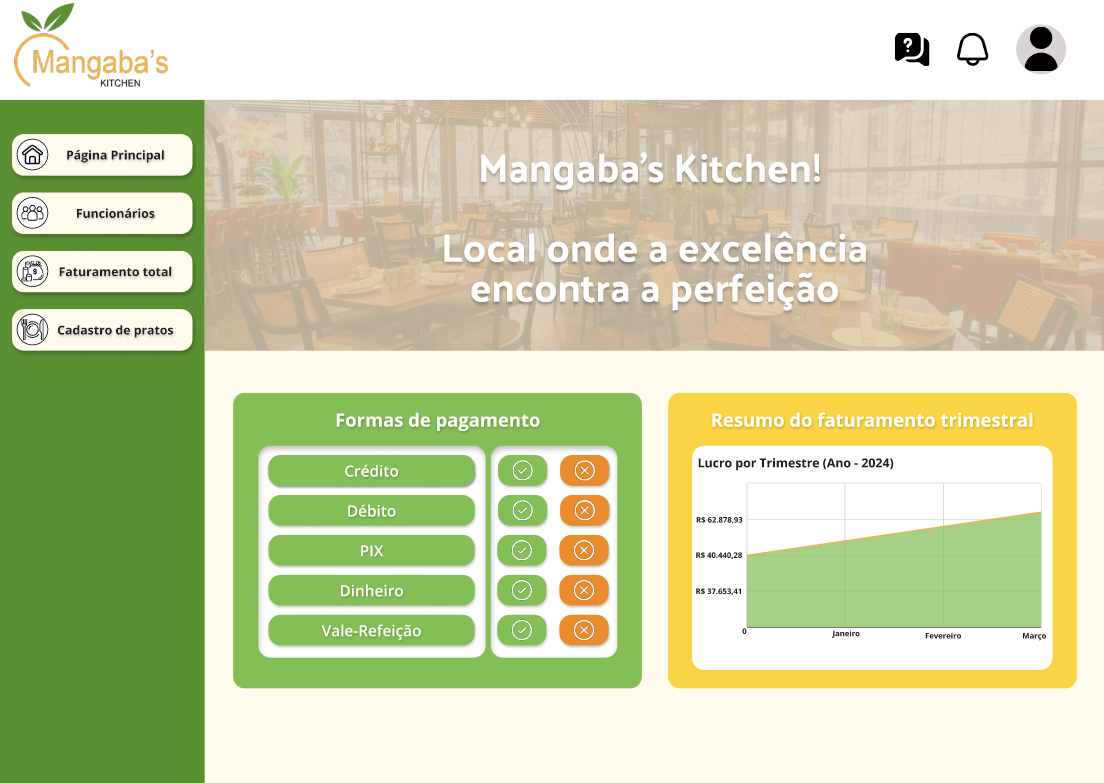
\includegraphics[width=1\textwidth]{imagens-template/Layout_Gerente_2700.png} 
        \caption{Painel inicial do gerente, com gerenciamento dos meios de pagamento e um gráfico trimestral do faturamento do restaurante.}
    \end{figure}
    \newpage
    \begin{figure}[!htp]
        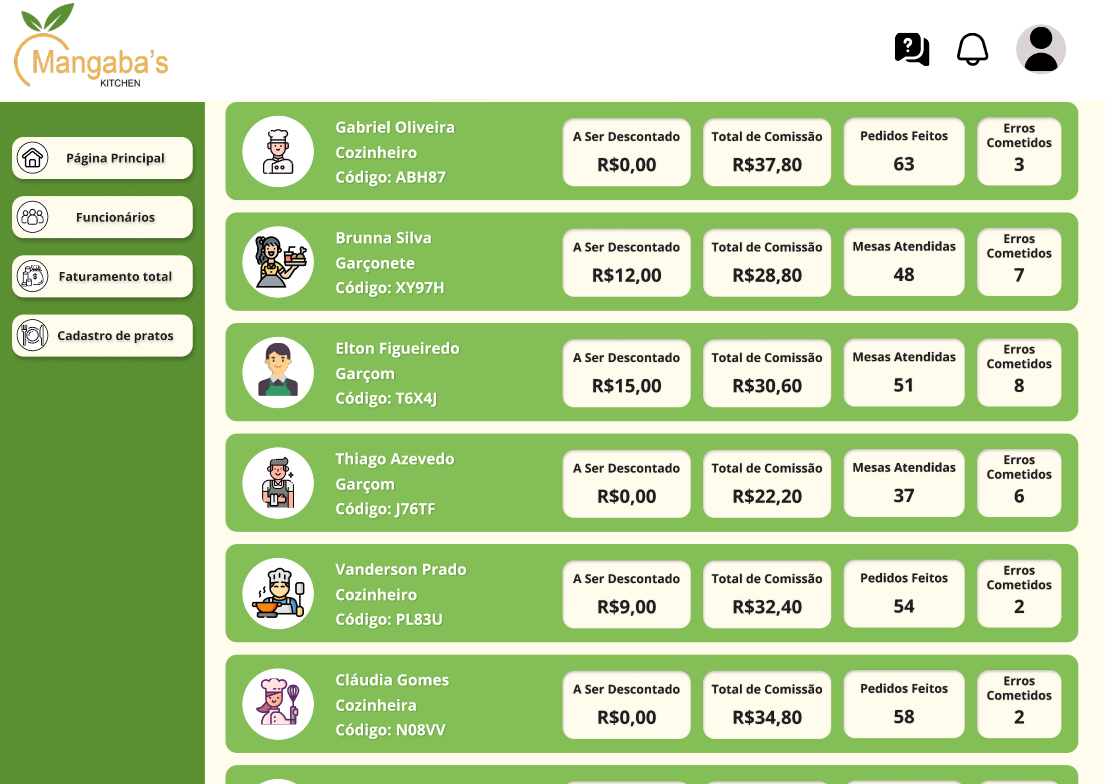
\includegraphics[width=1\textwidth]{imagens-template/Layout_Gerente_2659.png} 
        \caption{Painel de funcionários com as informações mais relevantes, como prejuízo causado e lucro gerado.}
    \end{figure}
    \newpage
    \begin{figure}[!htp]
        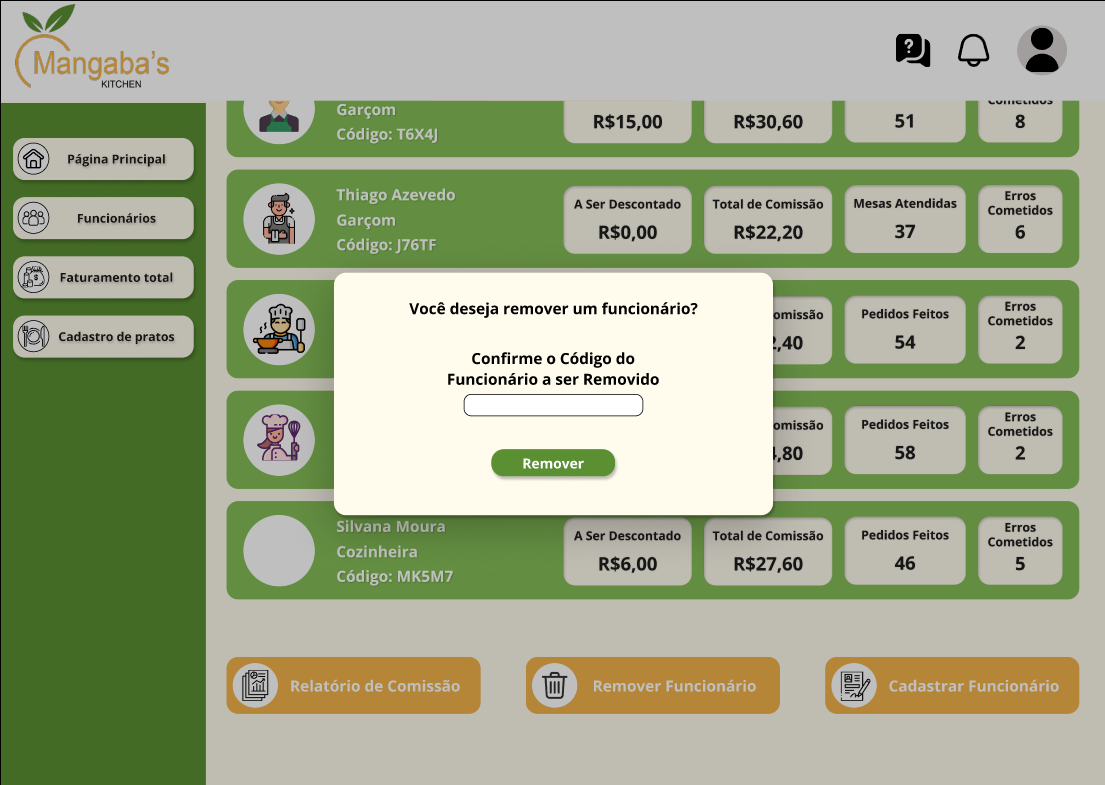
\includegraphics[width=1\textwidth]{imagens-template/Layout_Gerente_2657.png} 
        \caption{Pop-up de remoção de funcionário, pedindo o código como confirmação.}
    \end{figure}
    \newpage
    \begin{figure}[!htp]
        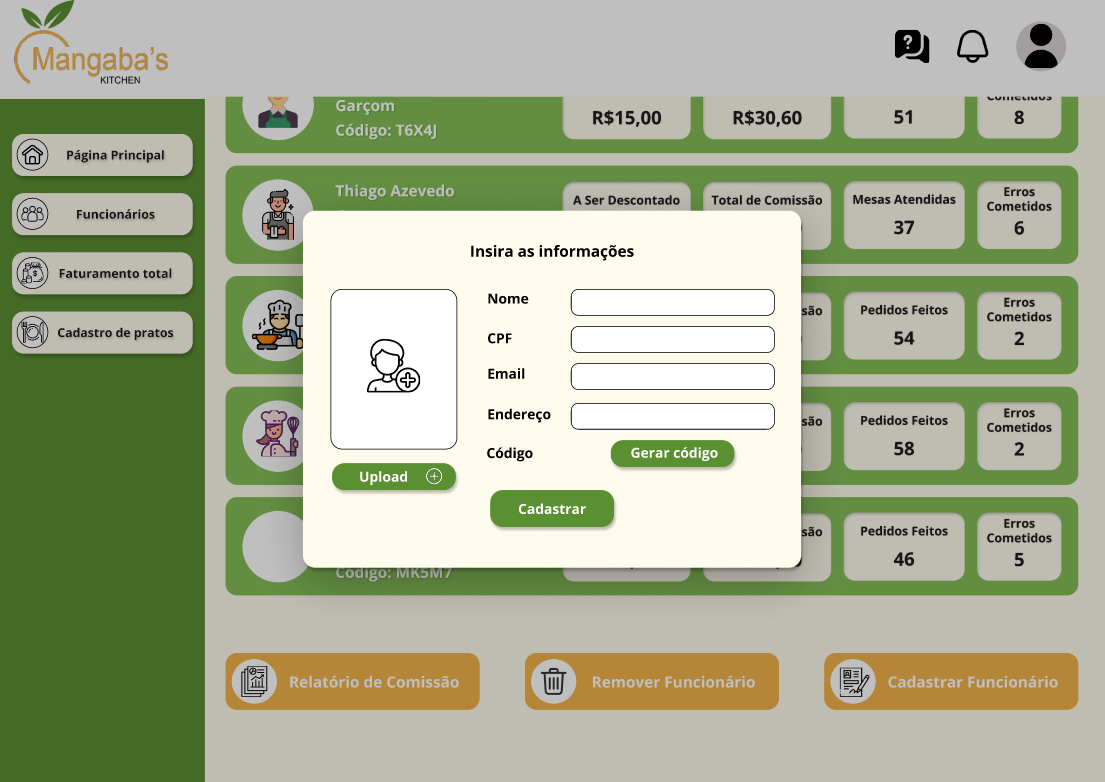
\includegraphics[width=1\textwidth]{imagens-template/Layout_Gerente_2655.png} 
        \caption{Pop-up de cadastro de funcionário, com os campos nome, cpf, email, endereço e um código gerado aleatóriamente, que se renova a cada 3 meses. Também há a opção do upload da foto do funcionário para melhor identificação.}
    \end{figure}
    \newpage
    \begin{figure}[!htp]
        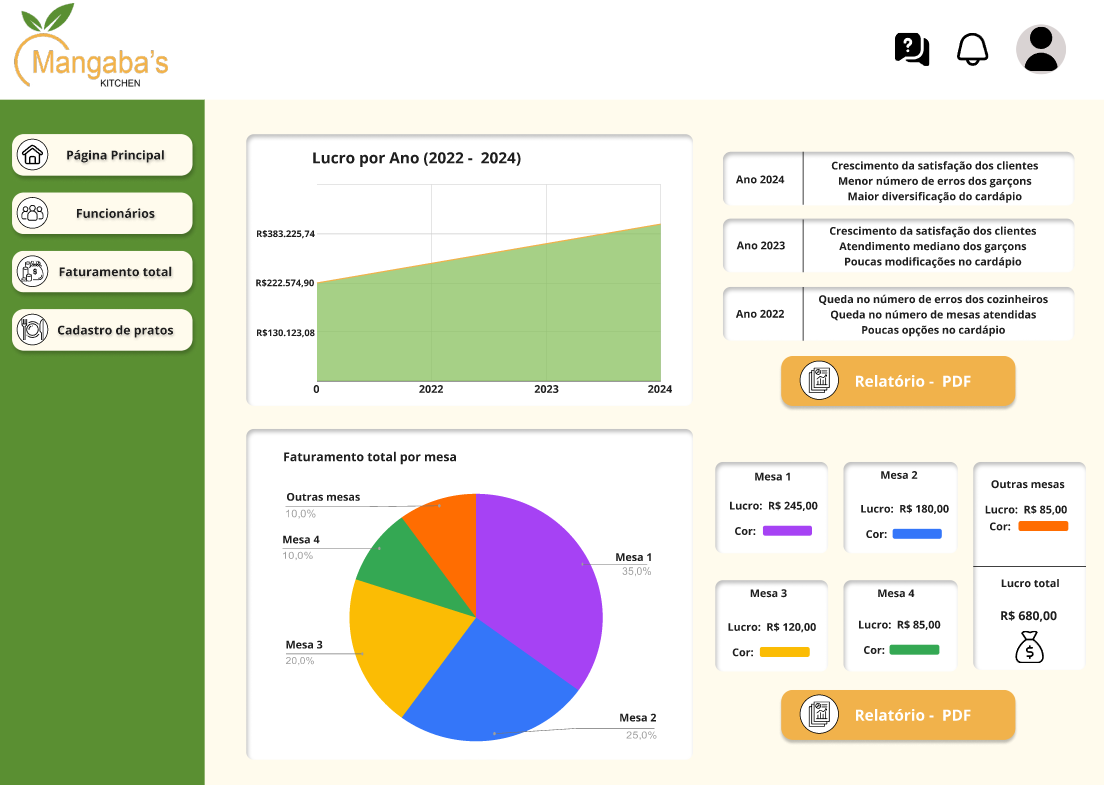
\includegraphics[width=1\textwidth]{imagens-template/Layout_Gerente_2653.png} 
        \caption{Tela de faturamento, com gráficos anuais e lucro por mesa, com uma definição construída pelo software e com opção para emissão de relatório.}
    \end{figure}
    \newpage
    \begin{figure}[!htp]
        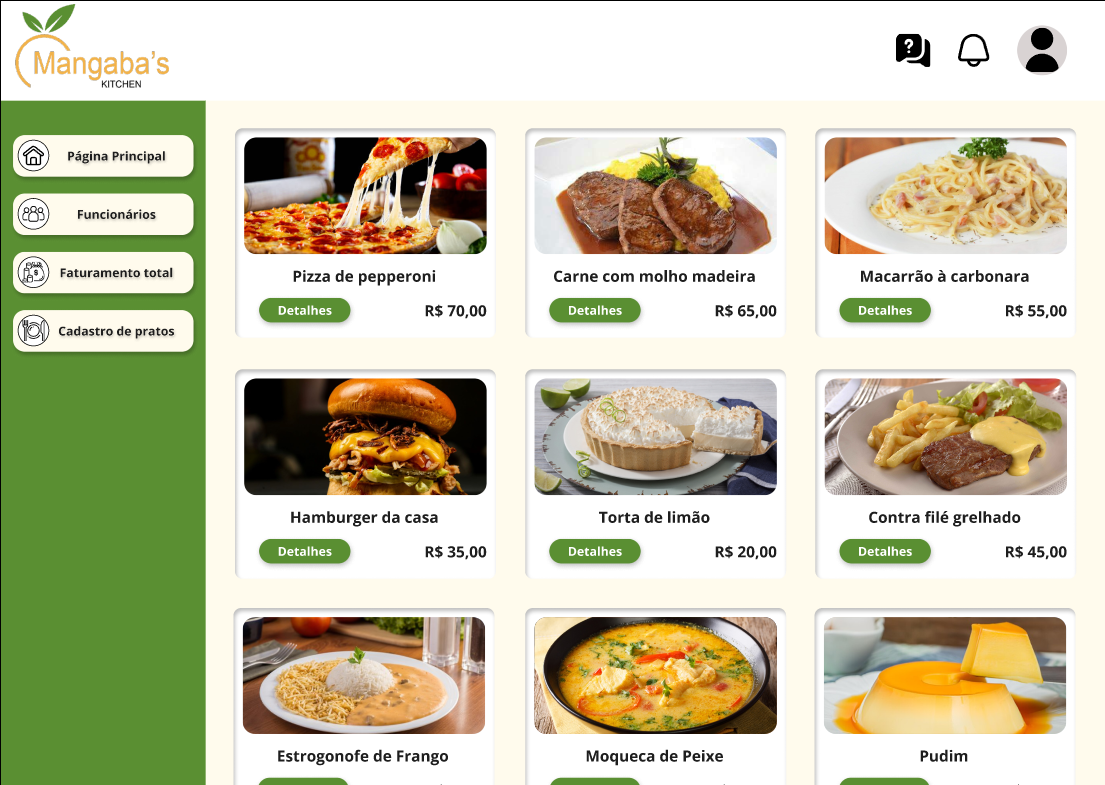
\includegraphics[width=1\textwidth]{imagens-template/Layout_Gerente_2651.png} 
        \caption{Painel de pratos cadastrados.}
    \end{figure}
    \newpage
    \begin{figure}[!htp]
        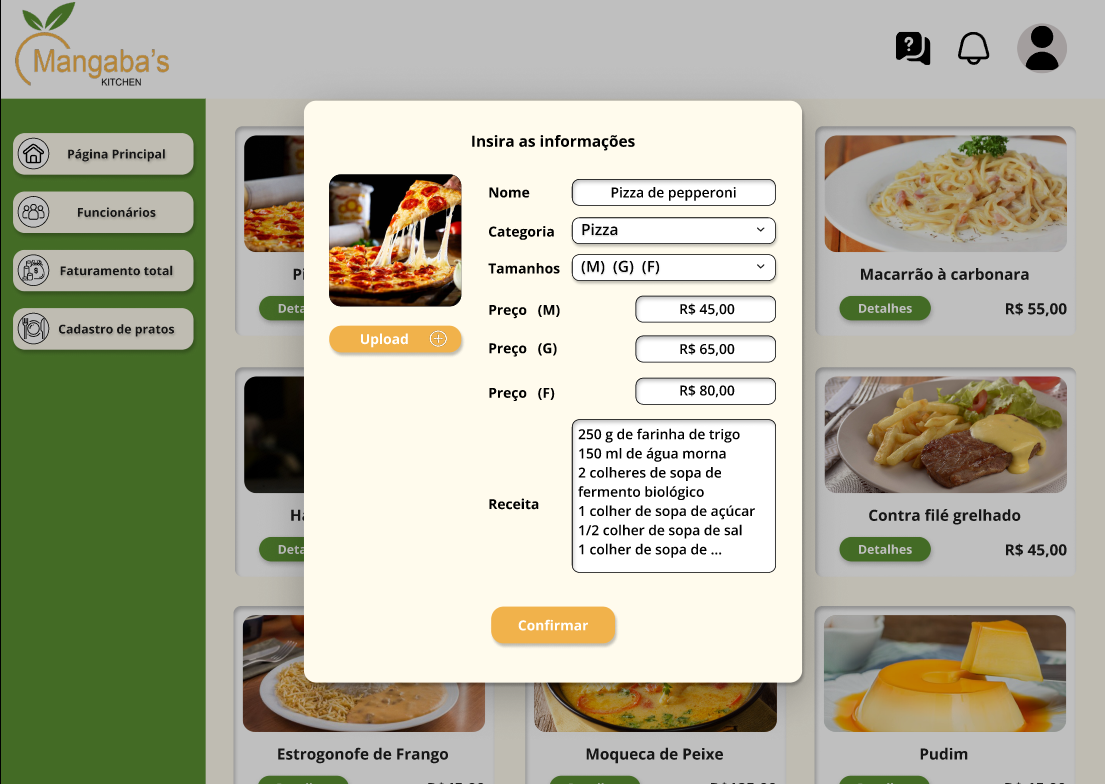
\includegraphics[width=1\textwidth]{imagens-template/Layout_Gerente_2649.png} 
        \caption{Pop-up de detalhes do prato, com possibilidade de alterar qualquer informação do prato. Se os campos ficarem em branco, o prato não será mostrado no painel.}
    \end{figure}
    \newpage
    \begin{figure}[!htp]
        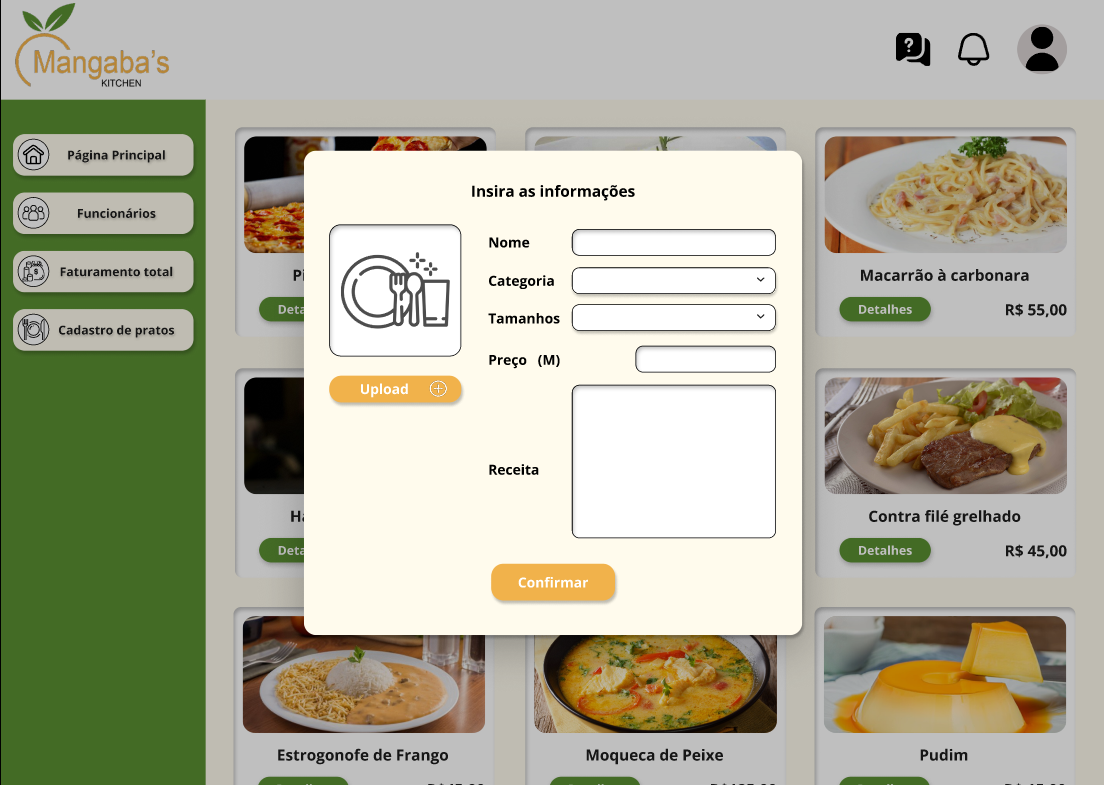
\includegraphics[width=1\textwidth]{imagens-template/Layout_Gerente_2647.png} 
        \caption{Pop-up de cadastro de prato, com opção para inserir uma imagem, selecionar o tamanho e o preço de cada tamanho disponível, além de um campo para inserir a receita. Se os campos ficarem em branco, o prato não será mostrado no painel.}
    \end{figure}
    \newpage
\end{center}

\newpage
\begin{center}
    \subsection{Telas do Garçom}
    \begin{figure}[!htp]
    \includegraphics[width=0.9\textwidth]{imagens-template/Layout_Garçom_2644.png} 
        \caption{Tela de login do funcionário.}
    \end{figure}
    \newpage
    \begin{figure}[!htp]
    \includegraphics[width=0.9\textwidth]{imagens-template/Layout_Garçom_2642.png} 
        \caption{Painel principal do garçom, com o controle de mesas ativas e inativas. Também a opção de consultar o histórico e cardápio.}
    \end{figure}
    \newpage
    \begin{figure}[!htp]
    \includegraphics[width=0.9\textwidth]{imagens-template/Layout_Garçom_2632.png} 
        \caption{Exemplo de uma mesa com pedido ativo. Há opções para inserir o modo de pagamento, nome do cliente, se é para levar ou não... Também é feita a soma de todos os itens no pedido e é mostrado para o garçom. Tem uma seção para verificar o status do pedido na cozinha e o tempo estimado para a finalização do prato. Mais abaixo são os itens do pedido e suas observações.}
    \end{figure}
    \newpage
    \begin{figure}[!htp]
    \includegraphics[width=0.9\textwidth]{imagens-template/Layout_Garçom_2629.png} 
        \caption{Pop-up para selecionar o meio de pagamento (Repare que a mesa está inativa).}
    \end{figure}
    \newpage
    \begin{figure}[!htp]
    \includegraphics[width=0.9\textwidth]{imagens-template/Layout_Garçom_2640.png} 
        \caption{Restante da página de mesa ativa, com o botão para adicionar mais itens ao pedido.}
    \end{figure}
    \newpage
    \begin{figure}[!htp]
    \includegraphics[width=0.9\textwidth]{imagens-template/Layout_Garçom_2634.png} 
        \caption{Consulta do cardápio que aparece quando o garçom precisa adicionar algum item no pedido. Os itens são separados em categorias.}
    \end{figure}
    \newpage
    \begin{figure}[!htp]
    \includegraphics[width=0.9\textwidth]{imagens-template/Layout_Garçom_2636.png} 
        \caption{Consulta individual do histórico de pedidos do garçom}
    \end{figure}
    \newpage
    \begin{figure}[!htp]
    \includegraphics[width=0.9\textwidth]{imagens-template/Layout_Garçom_2627.png} 
        \caption{Pop-up aberto ao clicar em "Detalhes", na aba de histórico. Aqui é mostrado ao usuário todas as informações sobre o pedido}
    \end{figure}
    \newpage
\end{center}

\begin{center}
    \subsection{Telas da Cozinha}
    \begin{figure}[!htp]
        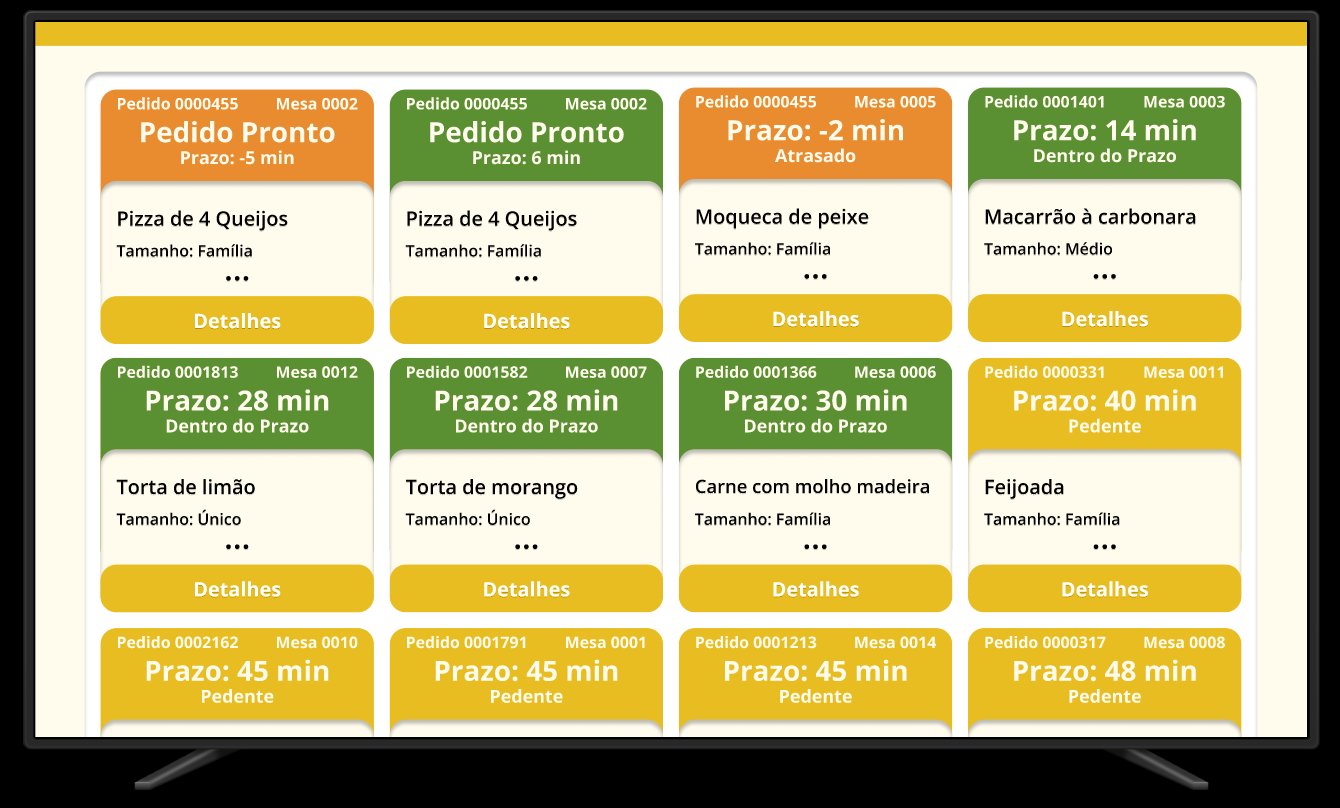
\includegraphics[width=1\textwidth]{imagens-template/Layout_Cozinha_2622.png}
        \caption{Painel da cozinha, mostrando o prazo para o pedido, se ele está pronto, o item daquele pedido, o número da mesa e o tamanho do item.}
    \end{figure}
    \newpage
    \begin{figure}[!htp]
        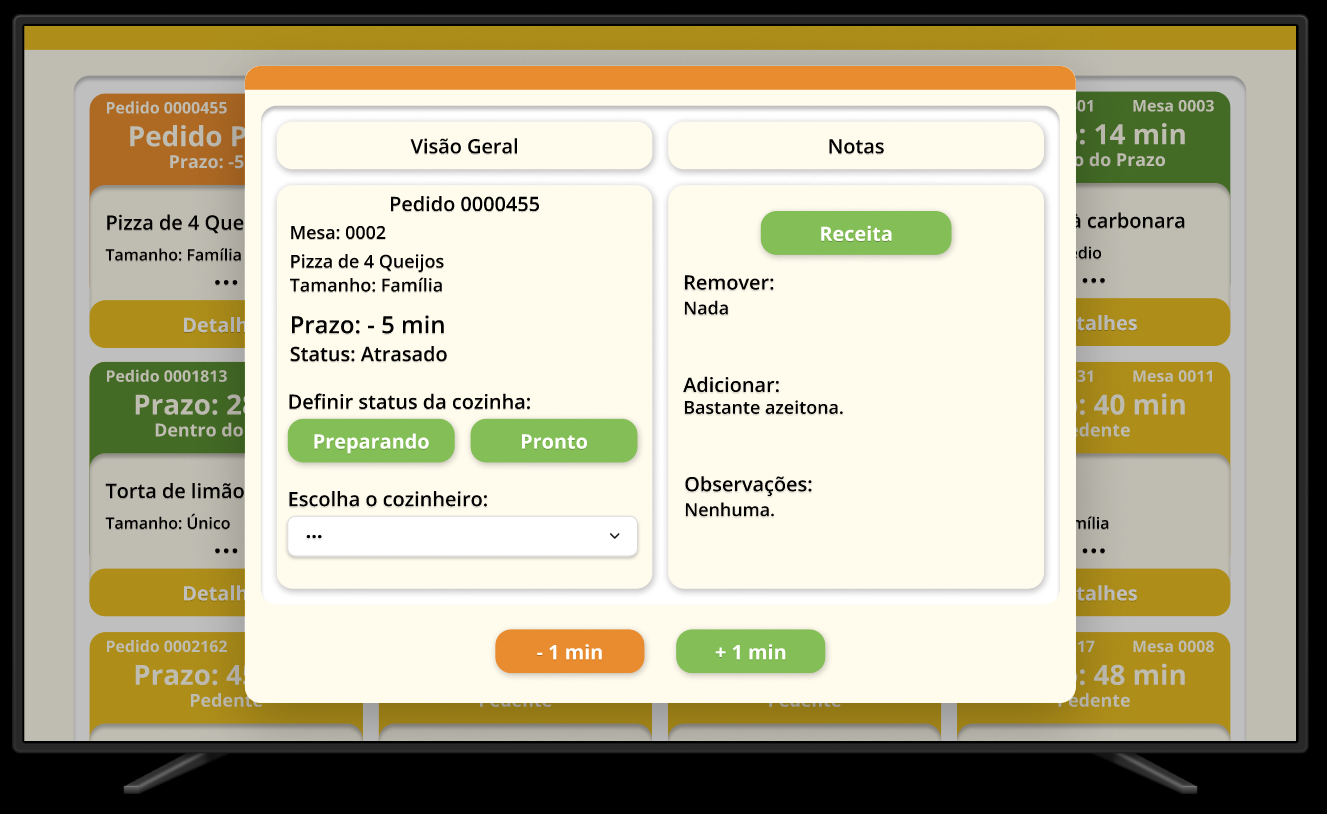
\includegraphics[width=1\textwidth]{imagens-template/Layout_Cozinha_2618.png}  
        \caption{Pop-ip de um pedido atrasado que foi aberto após o usuário clicar em "Detalhes" no painel principal. Aqui ele pode incrementar e decrementar o tempo, selecionar o cozinheiro responsável pelo pedido, e ver a receita do item.}
    \end{figure}
    \newpage
    \begin{figure}[!htp]
        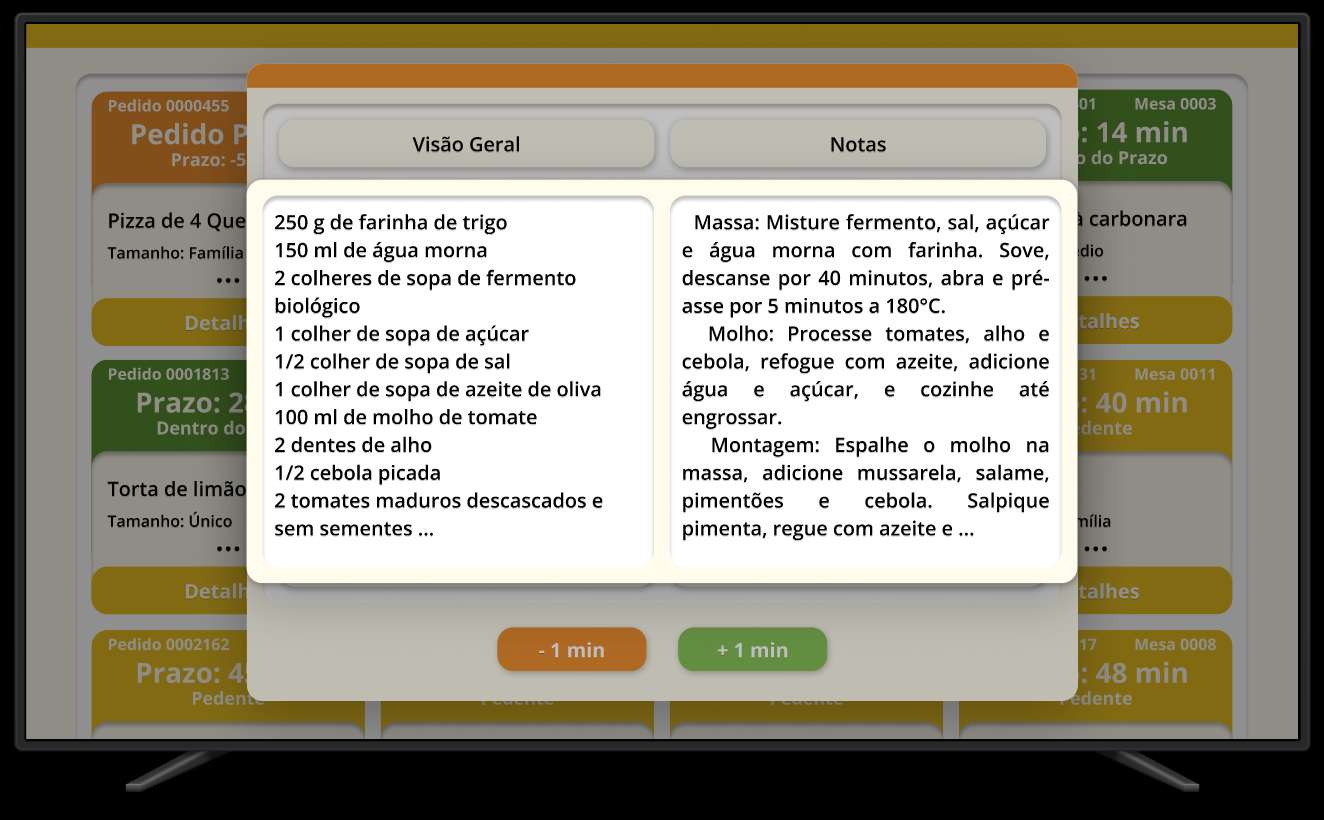
\includegraphics[width=1\textwidth]{imagens-template/Layout_Cozinha_2610.png} 
        \caption{Pop-up da receita do item}
    \end{figure} 
\end{center}